\subsection{Text}

\subsubsection{Title page without page number}

\begin{verbatim}
\clearpage\maketitle
\thispagestyle{empty}
\end{verbatim}

\subsubsection{Writing a comment}
\begin{figure}[h!]
\centering
\includegraphics[scale=0.4]{images/latex_comments.png}
\caption{\LaTeX comments}
\label{fig:comments}
\end{figure}

\subsubsection{Table of contents}
\begin{verbatim}
\tableofcontents
\end{verbatim}

\subsubsection{Danish characters}
\begin{verbatim}
\AA, \aa
\AE, \ae
\O, \o
\end{verbatim}
\AA, \aa \\*
\AE, \ae \\*
\O, \o

\clearpage

\subsection{Graphics}

\subsubsection{Caption over image}
\begin{verbatim}
\includegraphics[scale=0.4]{latex_comments.png}
\caption{\LaTeX comments}
\label{fig:f1}
\end{verbatim}

\subsubsection{Caption under image}
\begin{verbatim}
\caption{\LaTeX comments}
\includegraphics[scale=0.4]{latex_comments.png}
\end{verbatim}

\subsubsection{Label}
\begin{verbatim}
\label{fig:comments}
\end{verbatim}

\subsubsection{Centering}
\begin{verbatim}
\centering
\end{verbatim}

\subsubsection{Two images next to each other}

\begin{figure}[h!]
  \centering
  \subfloat[Version 1]{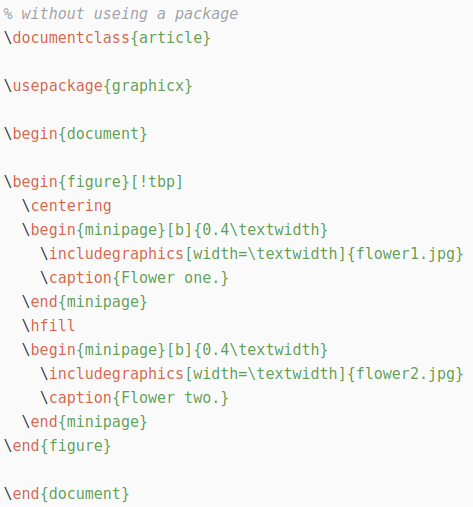
\includegraphics[width=0.4\textwidth]{images/image1.png}\label{fig:f2}}
  \hfill % is used for lining up the images in one row
  \subfloat[Version 2]{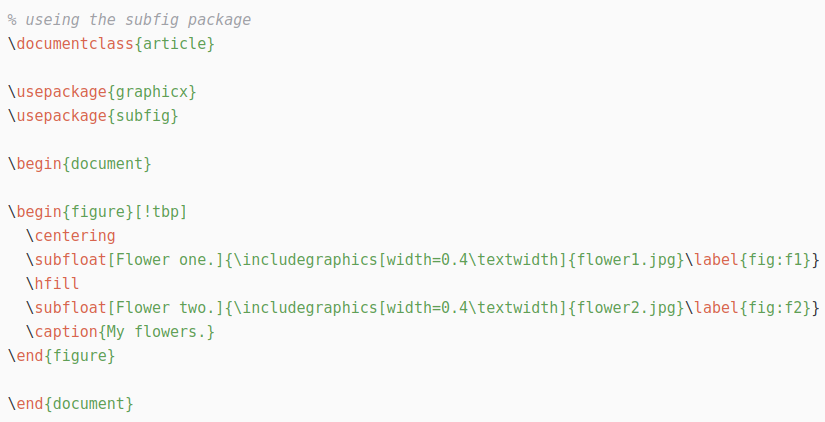
\includegraphics[width=0.4\textwidth]{images/image2.png}\label{fig:f3}}
  \caption{Images}
  \citep{stackexchange}
\end{figure}

\subsubsection{Reference to image}
\begin{verbatim}
\citep{here comes the name of the reference in the bib file}
Reference is shown at the last page.
\end{verbatim}

\subsubsection{Reference to page containing the image}
\begin{verbatim}
see figure \ref{fig:f2} on page \pageref{fig:f2}
\end{verbatim}

\clearpage

\subsection{Lists and Sections}

\subsubsection{Numbered Section}
\begin{verbatim}
\section{First Section}
\section{Second Section}
\end{verbatim}


\subsubsection{Non-Numbered Section}
\begin{verbatim}
\section*{First Section}
\section*{Second Section}
\end{verbatim}

\subsubsection{Bullet points}
\begin{verbatim}
\begin{itemize}
    \item Milk
    \item Sugar
\end{itemize}
\end{verbatim}

\subsubsection{Alternative bullet symbols}
\begin{verbatim}
\renewcommand{\labelitemi}{$\blacksquare$}
\renewcommand\labelitemii{$\square$}
\begin{itemize}
  \item  Milk
  \item  Sugar
\end{itemize}
\end{verbatim}

\subsubsection{Enumerated lists}
\begin{verbatim}
\begin{enumerate}
    \item Milk
    \item Sugar
\end{enumerate}
\end{verbatim}

\subsubsection{Roman numerals, letters}
\paragraph{Roman numbers in enumerate list}
\begin{verbatim}
\begin{enumerate}[label=(\Roman*)]
  \item  Milk
  \item  Sugar
\end{enumerate}
\end{verbatim}

\paragraph{Letters in enumerate list}
\begin{verbatim}
\begin{enumerate}[label=(\roman*)]
  \item  Milk
  \item  Sugar
\end{enumerate}
\end{verbatim}

\subsection{Table with multiple columns}

\subsubsection{Various horizontal alignments in columns (left, right, centered)}

\begin{table}[htp]
    \centering
\begin{tabular}{ | l | c | r | }
\hline
  Left & Center & Right \\ \hline
  Left and Left & Center and Center & Right and Right \\ \hline
  Left & Center & Right \\
\hline
\end{tabular}
    \caption{Caption}
    \label{tab:my_label_1}
\end{table}



\subsubsection{Cell spanning multiple columns}
\begin{table}[htp]
    \centering
    \begin{tabular}{|r|l|}
    \hline
     7C0 & hexadecimal \\
     3700 & octal \\ \cline{2-2}
     11111000000 & binary \\
     \hline \hline
     1984 & decimal \\
    \hline
    \end{tabular}
    \caption{Caption}
    \label{tab:my_label_2}
\end{table}

\subsubsection{Vertical alignment in multi-line cells}


\begin{table}[htp]
    \centering
\begin{tabular}{ |l|l| }
  \hline
  \multicolumn{2}{|c|}{Team sheet} \\
  \hline
  GK & Paul Robinson \\
  LB & Lucas Radebe \\
  DC & Michael Duberry \\
  DC & Dominic Matteo \\
  RB & Dider Domi \\
  MC & David Batty \\
  MC & Eirik Bakke \\
  MC & Jody Morris \\
  FW & Jamie McMaster \\
  ST & Alan Smith \\
  ST & Mark Viduka \\
  \hline
\end{tabular}
    \caption{Caption}
    \label{tab:my_label_3}
\end{table}


\subsubsection{Table description and label}
\begin{verbatim}
    \caption{Description}
    \label{tab:my_label_3}
\end{verbatim}

\subsubsection{Reference to table}
Table~\ref{tab:my_label_1} summarizes Text
\newline
Table~\ref{tab:my_label_2} summarizes Text
\newline
Table~\ref{tab:my_label_3} summarizes Text
\newline
\begin{verbatim}
    Table~\ref{tab:my_label_1} summarizes Text \\
    Table~\ref{tab:my_label_2} summarizes Text \\
    Table~\ref{tab:my_label_3} summarizes Text \\
\end{verbatim}


\subsection{Code listing}

\subsubsection{With emphasized key words in your favorite programming language}

\begin{lstlisting}
// Hello.java
import javax.swing.JApplet;
import java.awt.Graphics;

public class Hello extends JApplet {
    public void paintComponent(Graphics g) {
        g.drawString("Hello, world!", 65, 95);
    }    
}
\end{lstlisting}

\subsection{Math equations}

\subsubsection{Inline equations (in text)}

The well known Pythagorean theorem \(x^2 + y^2 = z^2\) was 
proved to be invalid for other exponents.

\subsubsection{Display equations (on separate line)}

This is a simple math expression
\[\sqrt{x^2+1}\] 
separated from text.

\subsubsection{Numbered equation}
\begin{equation}
E=m
\end{equation}

\subsubsection{Fractions, summations, products, roots, powers}

\begin{enumerate}
    \item \(\frac{1}{2}\)
    \item \(x + y = z\)
    \item \(x * y = z\)
    \item \(\sqrt{x^2+1}\) 
    \item \begin{math}{x^2}\end{math}
    \item \({x^3}\)
\end{enumerate}

\subsection{Bibliography with book, article and internet link}
\subsubsection{Hyperlinks}
\href{http://www.sharelatex.com}{Something Linky}
\begin{verbatim}
\href{http://www.sharelatex.com}{Something Linky}
\end{verbatim}
    
\subsubsection{Bibliography and article}
Bibliographic references are usually kept in a bibliography file whose extension is .bib, this file consists of a list of records and fields. Each bibliography record holds relevant information for a single entry. 


\begin{verbatim}
@article{einstein,
    author =       "Albert Einstein",
    title =        "{Zur Elektrodynamik bewegter K{\"o}rper}. ({German})
        [{On} the electrodynamics of moving bodies]",
    journal =      "Annalen der Physik",
    volume =       "322",
    number =       "10",
    pages =        "891--921",
    year =         "1905",
    DOI =          "http://dx.doi.org/10.1002/andp.19053221004"
}
\end{verbatim}

\subsection{To-do notes of own choice}

\paragraph{see the bottom of the page for the TO-DO note list}

\todo[inline]{The original to-do note without changed colours.\newline Here's another line.}
\lipsum[11]\unsure{Is this correct?}\unsure{I'm unsure about also!}
\lipsum[11]\change{Change this!}
\lipsum[11]\info{This can help me in chapter seven!}
\lipsum[11]\improvement{This really needs to be improved!\newline\newline What was I thinking?!}
\lipsum[11]
\thiswillnotshow{This is hidden since option `disable' is chosen!}
\improvement[inline]{The following section needs to be rewritten!}
\lipsum[11]
\newpage